\documentclass[a4paper,12pt]{article}
\usepackage[utf8]{inputenc}
\usepackage{amsmath}
\usepackage{graphicx}
\usepackage{geometry}
\usepackage{hyperref}
\geometry{a4paper, margin=1in}

\title{Evaluation von Photogrammetrie 3D Scan für CFD Simulationen}
\author{Peter Kuhn}
\date{2024-05-26}

\begin{document}

\maketitle

\tableofcontents

\section{Einleitung}\label{sec:Einleitung}
Das Ziel ist es zu bewerten, wie geeignet ein Photogrammetrie 3D-Scan für eine CFD-Simulation ist.

Dazu wird eine Simulation mit 3D-gescannten Objekten und eine Simulation mit den Originaldimensionen des Objekts gemacht.

Als Objekt wurde die Kuh gewählt. Fur vielen Beispielen der theoretischen Physik ist die Annahme, dass eine Kuh sphärisch ist, typisch. Im Jahr 2015 gab es das Meme das den Luftwiderstands einer Kuh mit dem eines Jeeps verglichen hat. Um diesen Witzen Ehre zu tragen, ist es das Ziel, den \( c_d \)-Wert einer Kuh zu ermitteln.

\newpage

\begin{figure}[h]
    \centering
    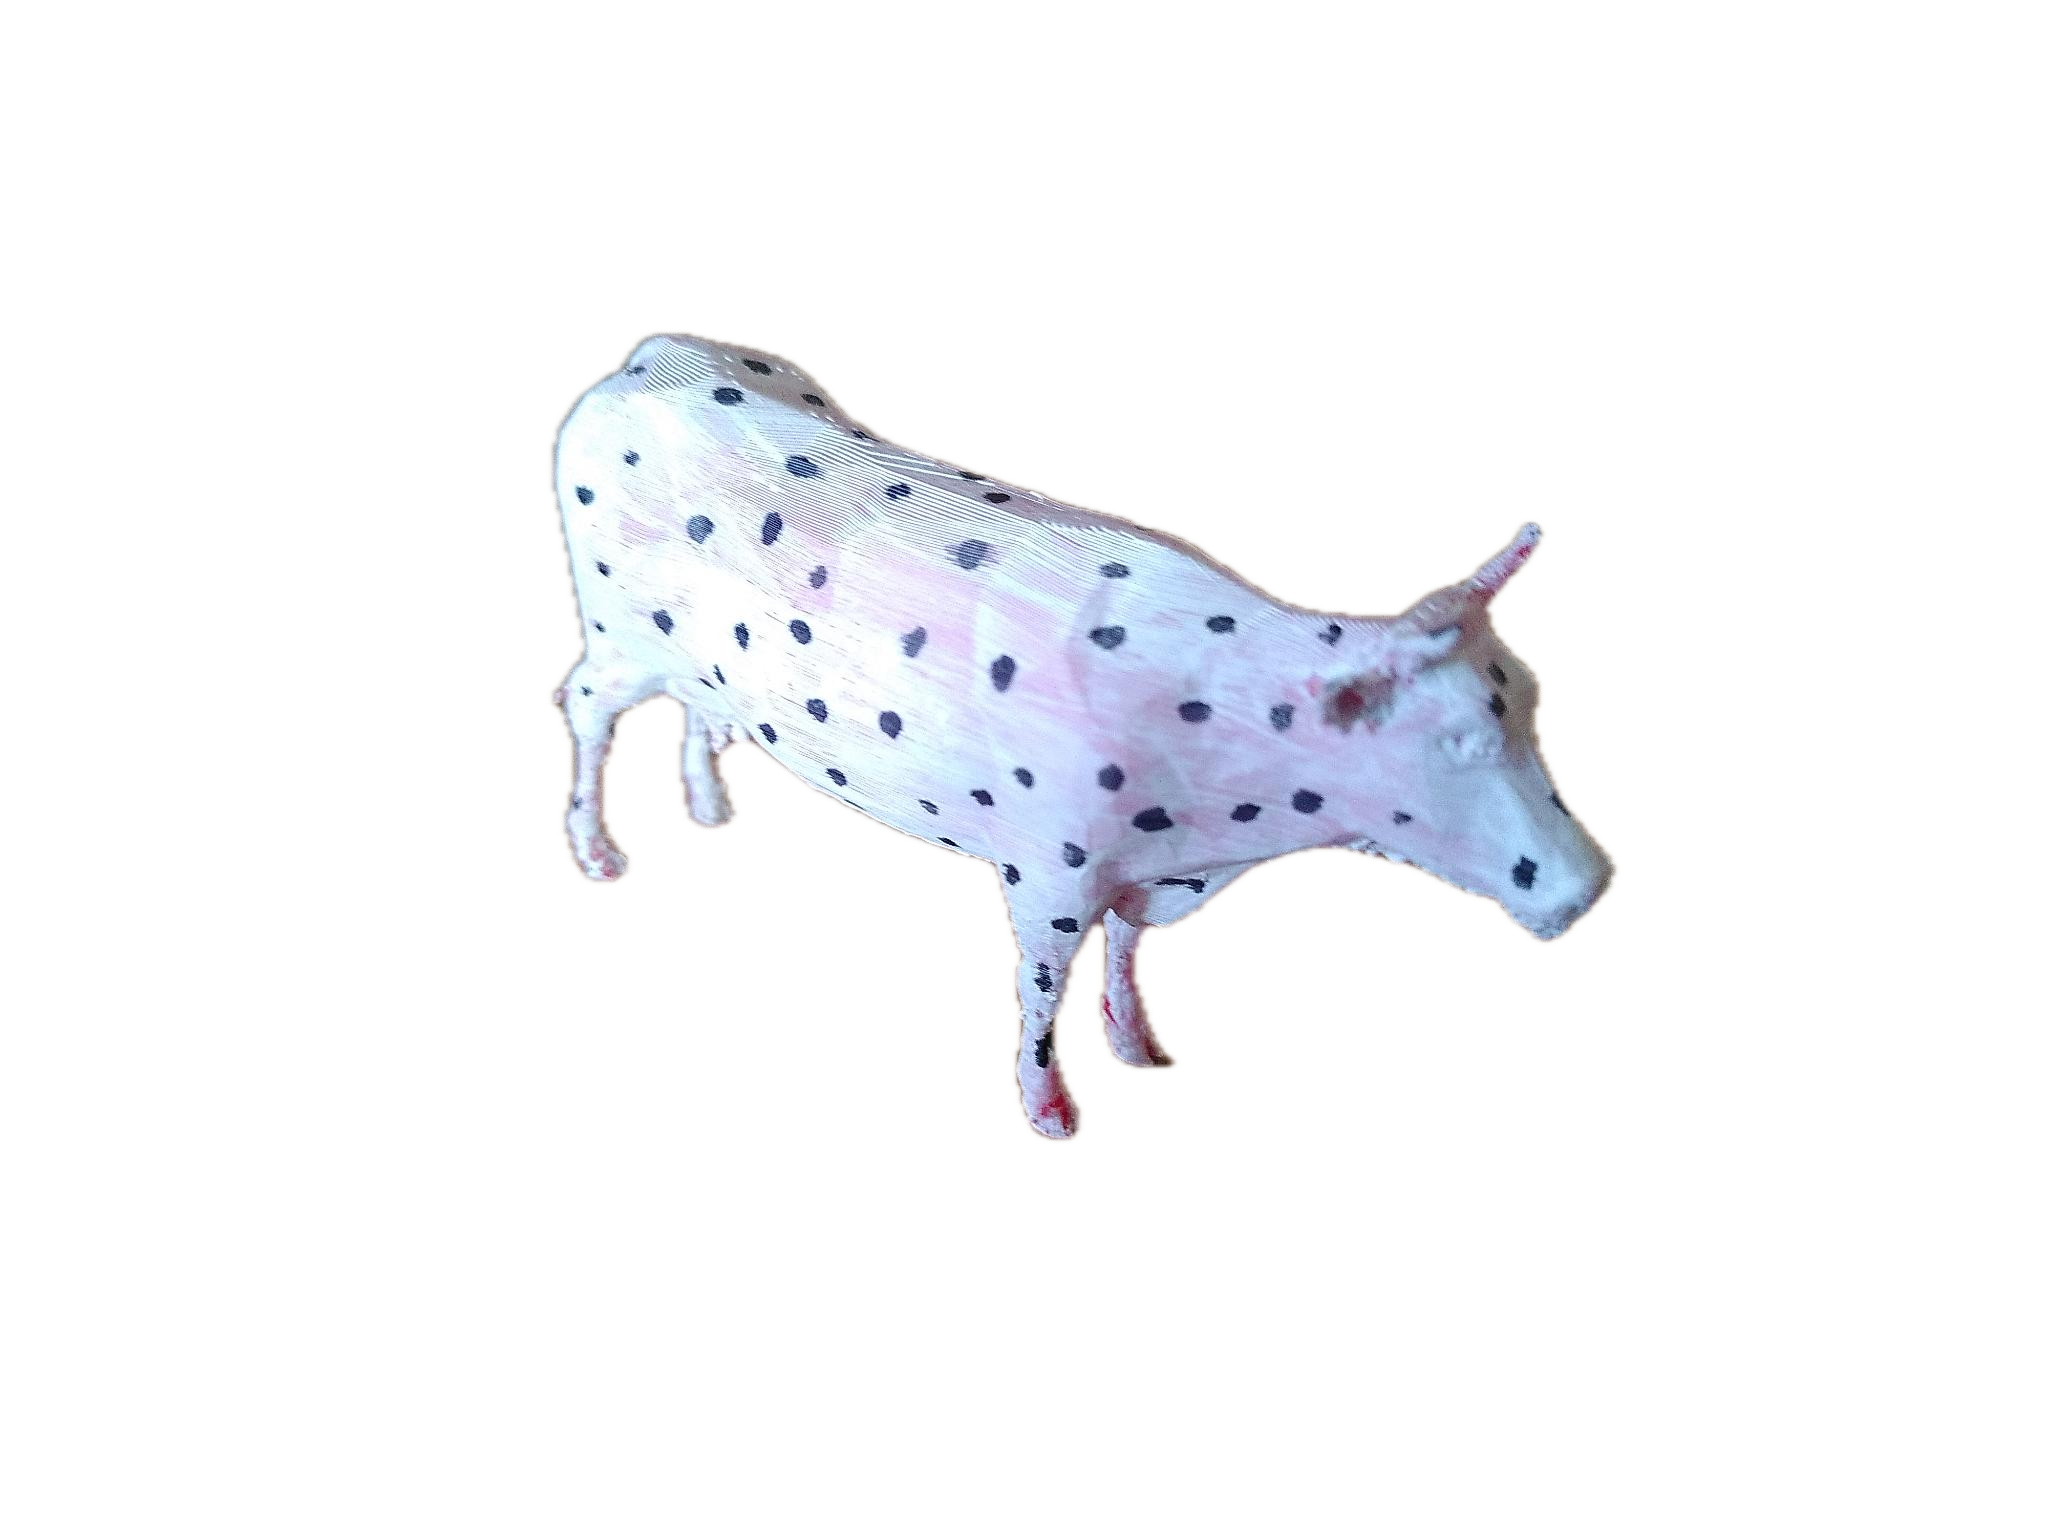
\includegraphics[width=0.5\textwidth]{signal-2024-05-26-124612.png}
    \caption{3D gedruckte Kuh, angemahlt}
    \label{fig:cowObj}
\end{figure}



Der Widerstandsbeiwert \( c_d \) ist definiert als

\begin{equation}
c_d = \frac{2 F_d}{\rho u^2 A}
\end{equation}

wobei:
\begin{itemize}
    \item \( F_d \) die Widerstandskraft ist, die per Definition die Kraftkomponente in Richtung der Strömungsgeschwindigkeit ist;
    \item \( \rho \) die Massendichte des Fluids ist;
    \item \( u \) die Strömungsgeschwindigkeit des Objekts relativ zum Fluid ist;
    \item \( A \) die Referenzfläche ist.
\end{itemize}

\section{Aufbau}

\subsection{Geometrie}
Um einen Vergleich der Geometrie zu machen, braucht es zwei Geometrien. Hierfür wurde zum einen eine frei verfügbare Low-Poly-Kuh und zum anderen der Scan des 3D-Drucks der Low-Poly-Kuh gemacht.

\begin{figure}[h]
    \centering
    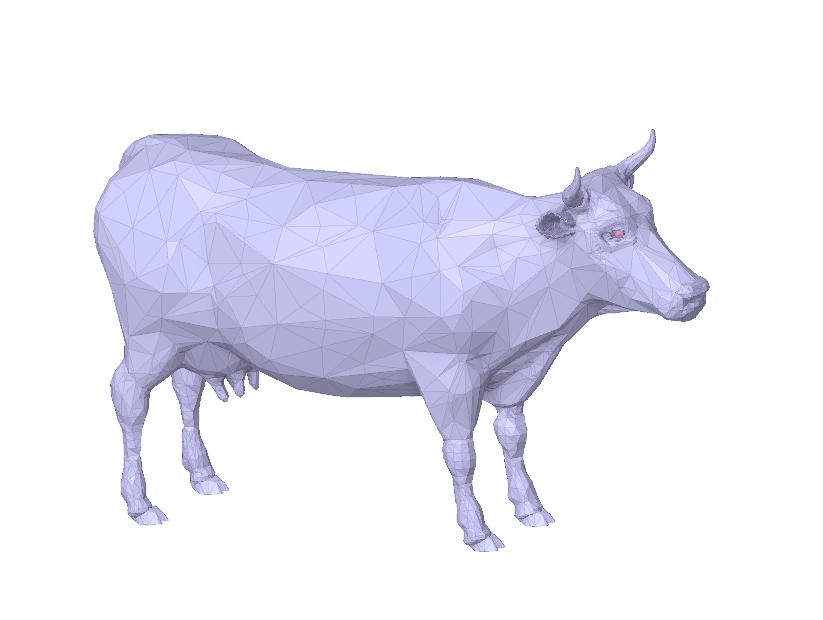
\includegraphics[width=0.5\textwidth]{cow.PNG}
    \caption{Orginal STL aus dem Internet}
    \label{fig:Orggeometry}
\end{figure}

\subsection{3D Scan Work Flow}
Um die gescannte Geometrie zu bekommen, wurden verschiedene Techniken ausprobiert. Hier ist der funktionierende Ablauf beschrieben:
\begin{enumerate}
    \item STL 3D-Datei im Internet finden \href{https://www.printables.com/de/model/175429-cow}{Kuh}
    \item Mit Prusa Slicer das STL in G-Code übersetzen
    \item Mit 3D-Drucker Ultimaker 2+ G-Code in physisches Objekt umwandeln
    \item 3D-Druck weiß und schwarz anmalen, um Reflexionen zu vermeiden und Tracking-Punkte zu setzen
    \item Mit Smartphone und externen LEDs mit der Software Polyscan 130 Bilder auf externen Servern in OBJ-Datei erstellen und exportierne
    \item Mit Blender OBJ bearbeiten, Boden entfernen, als STL exportieren
    \item In ANSYS Spaceclaim mit der Funktion Shrinkwrap ein zusammenhängenden STL erstellen
    \item In nTop aus STL eine implizite Geometrie erstellen
    \item In nTop aus impliziter Geometrie eine Konstruktion ableiten als STEP
    \item In NX die Konstruktion der Luft um die Kuh als prt Abbildung \ref{fig:nx} erstellen und als STEP exportieren
    \item In ANSYS importieren und vernetzen  
\end{enumerate}
Dieser Prozess ist schwierig, weil es keine universell einsetzbaren 3D-Dateiformate gibt. Ich hoffe, dass sich hier in der Zukunft etwas verbessert.


\begin{figure}[h]
    \centering
    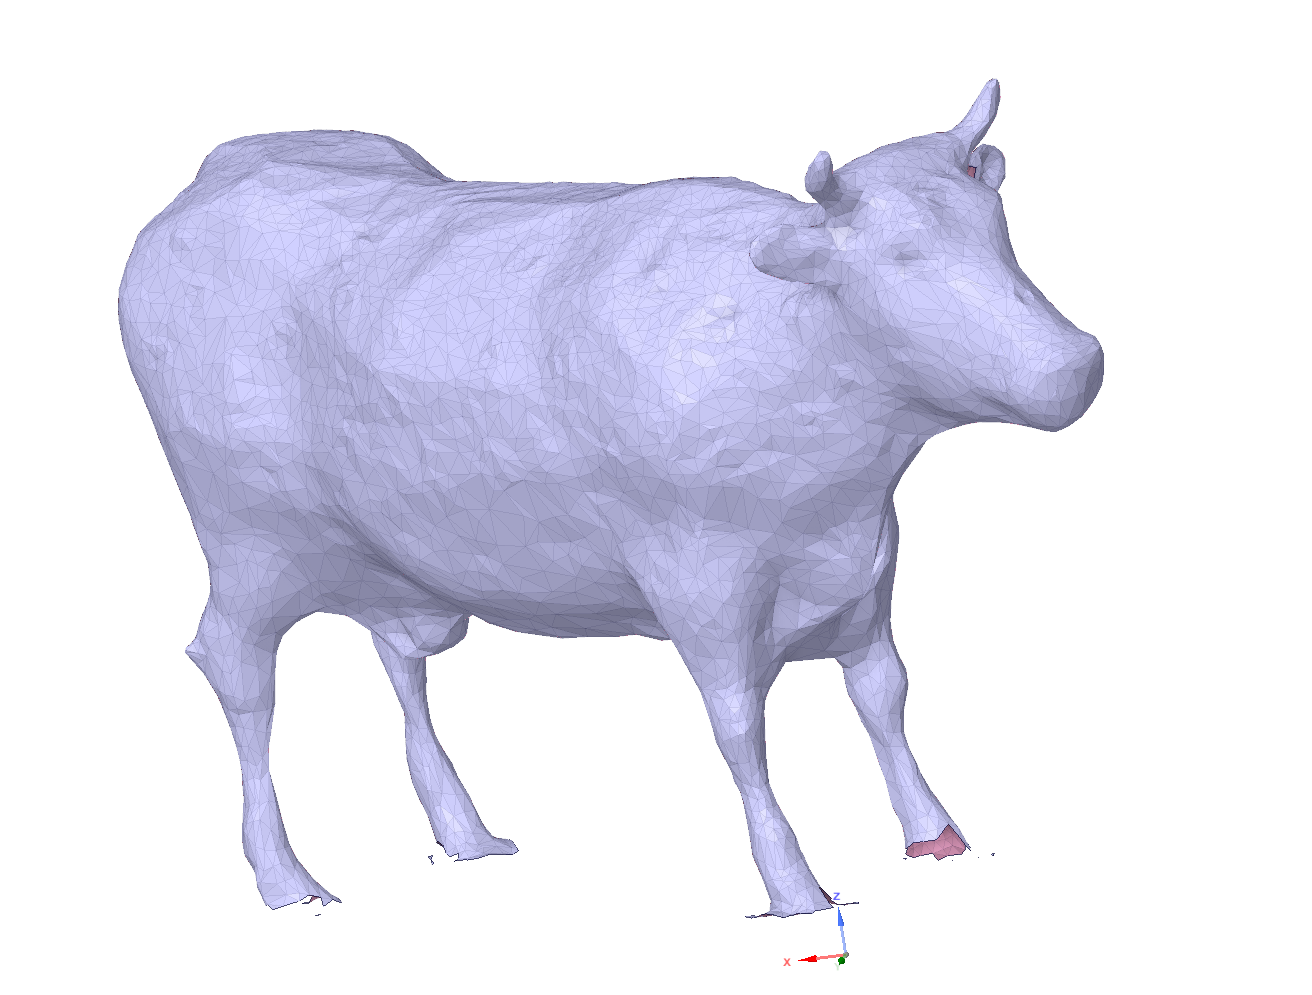
\includegraphics[width=0.5\textwidth]{cew.PNG}
    \caption{3D Scan nach Shrinkwrap, die Euter sind zum beispiel nicht mehr abgebieldet}
    \label{fig:scangeometry}
\end{figure}

\begin{figure}[h]
    \centering
    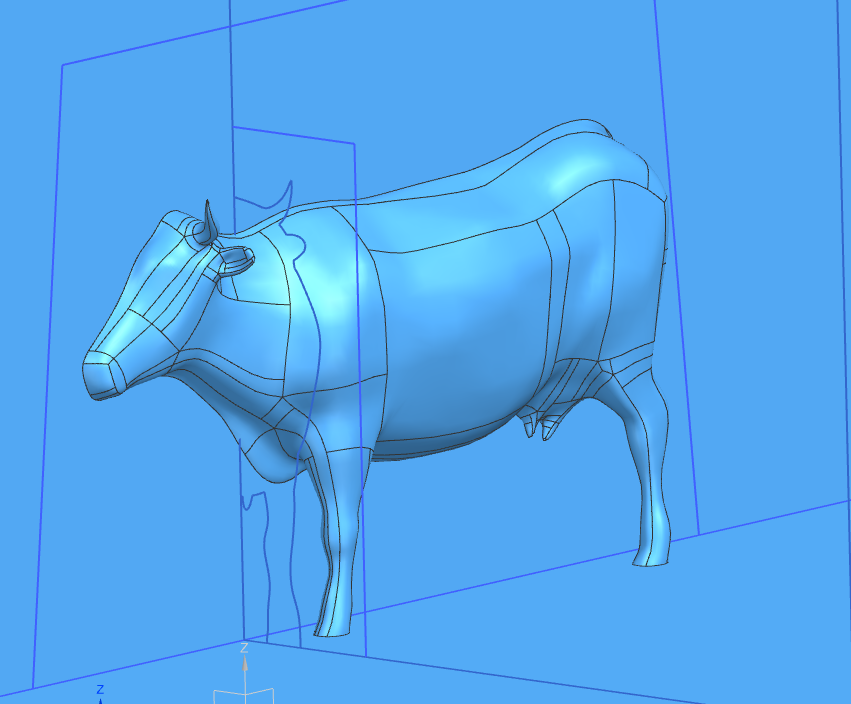
\includegraphics[width=0.5\textwidth]{nx.PNG}
    \caption{Die orginal Geometrie als prt in NX}
    \label{fig:nx}
\end{figure}

\subsection{Material}
Es wird Luft bei 25 Grad an einem schönen Frühlingstag für die Simulation gewählt.

\subsection{Randbedingungen}
Die \( c_d \) in der Literatur sind bei einer Reynolds-Zahl zwischen \( 10^4 \) und \( 10^6 \) angegeben. Das heißt, die Luftgeschwindigkeit \( u \) wird so gewählt, dass die Reynolds-Zahl passt.

Für die Simulation kann die Symmetrie der Kuh genutzt werden. Die Kuh ist als Wall no slip definiert, die Wände als Wall free slip, Inlet ist mit einer konstanten Geschwindigkeit definiert, Outlet ist als 0 Pa Druck definiert. 

\subsection{Handrechnung}\label{sec:handrechnung}
Für die Handrechnung wird die Annahme aus \ref{sec:Einleitung} benutzt. Der \( c_d \)-Wert einer Sphäre kann in der \href{https://en.wikipedia.org/wiki/Drag_coefficient}{Literatur} nachgeschlagen werden und ist
$$c_d = 0.47$$


\section{Vorstudien}

Die Expression, die als Monitorpunkt benutzt wird, ist
$$ force_y@cow$$

\begin{figure}[h]
    \centering
    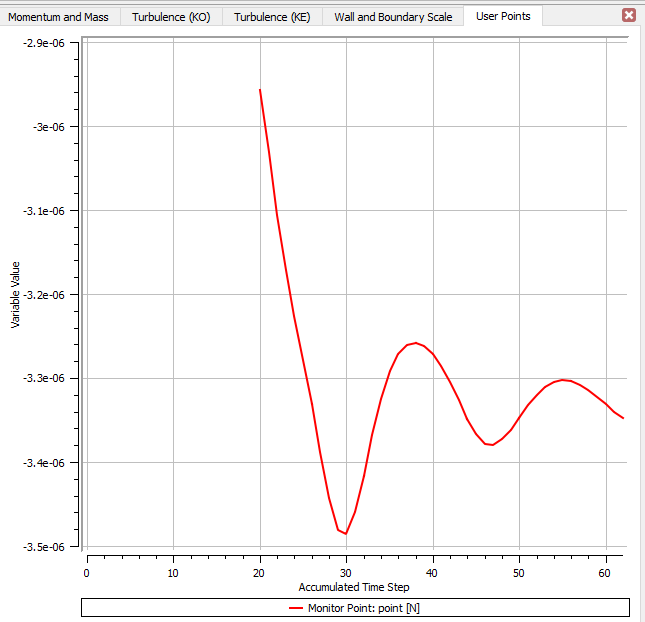
\includegraphics[width=0.5\textwidth]{force.PNG}
    \caption{Kraft auf die Flache der Kuh}
    \label{fig:F}
\end{figure}

Auch in Abblindung \ref{fig:F} kann gesehen werden, dass es sich leider nicht um eine laminare Strömung handelt. Um einen Wert zu bekommen, der mit dem Wert aus \ref{sec:handrechnung} verglichen werden kann, wird der Durchschnitt in den letzten Schwingungen ausgewertet.

Um die Referenzfläche A der Kuh zu erhalten, wird in NX ein Schatten der Kuh gemessen. In \ref{fig:A} ist zu sehen, dass zum beispiel nicht mehr berücksichtigt wird, dass eine Kuh Vorder- und Hinterbeine hat.


\begin{figure}[h]
    \centering
    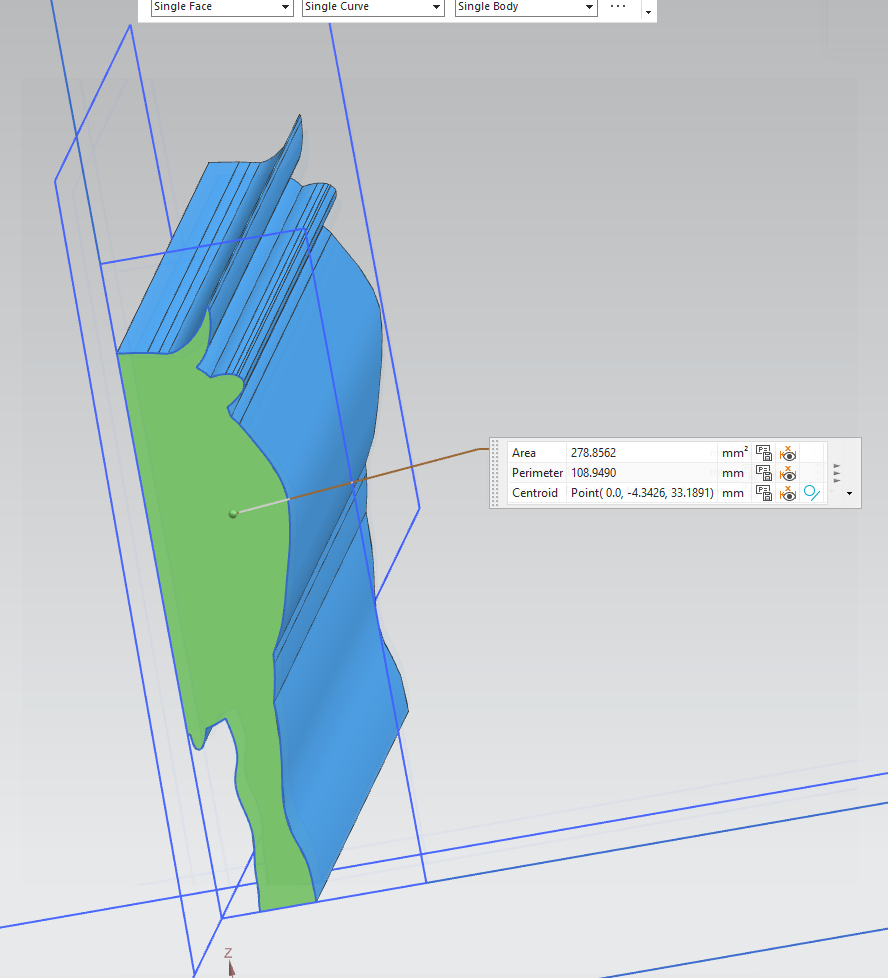
\includegraphics[width=0.5\textwidth]{surface.PNG}
    \caption{Referenzflache der Kuh}
    \label{fig:A}
\end{figure}

\subsection{Rechenintervalle}
Der RMS-Error in Abbildung \ref{fig:monitor1} ist nicht am konstanten Abnehmen, sondern zeigt die Eigenschaften einer Kármánschen Wirbelstraße. Meine Vermutung ist, dass die dünnen Beine der Kuh und der massige Körper der Kuh nicht die Vorgaben der Reynolds-Zahl und keine Wirbelablösung gleichzeitig aufweisen können.


\begin{figure}[h]
    \centering
    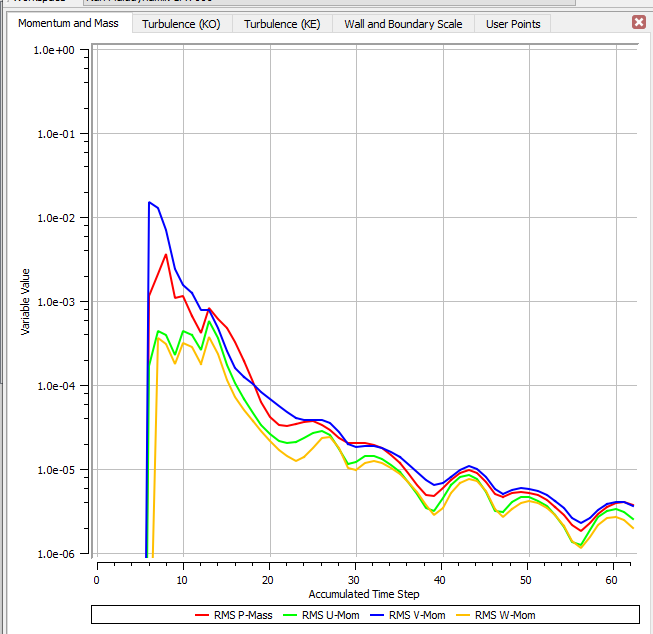
\includegraphics[width=0.5\textwidth]{rms.PNG}
    \caption{RMS Fehler, die nicht konvergieren}
    \label{fig:monitor1}
\end{figure}

\subsection{Grösse der simulierten Luft}
Um sicherzustellen, dass die Simulation eine Kuh auf freiem Feld abbildet, muss sichergestellt werden, dass die Wände der Simulation einen vernachlässigbaren grossen Einfluss auf das Ergebnis haben. Für die Evaluation des 3D-Scans wurde eine Größe gewählt, die dem Bauchgefühl nach ausreichend ist. Die Luft war für beide Simulationen genau gleich.

In dem Bild \ref{fig:p} kann gesehen werden, dass die Druckverteilung nicht bis an die Wänden inhomogen ist, das heißt, die wande haben tatsächlich keinen Einfluss auf die Kuh.

\begin{figure}[h]
    \centering
    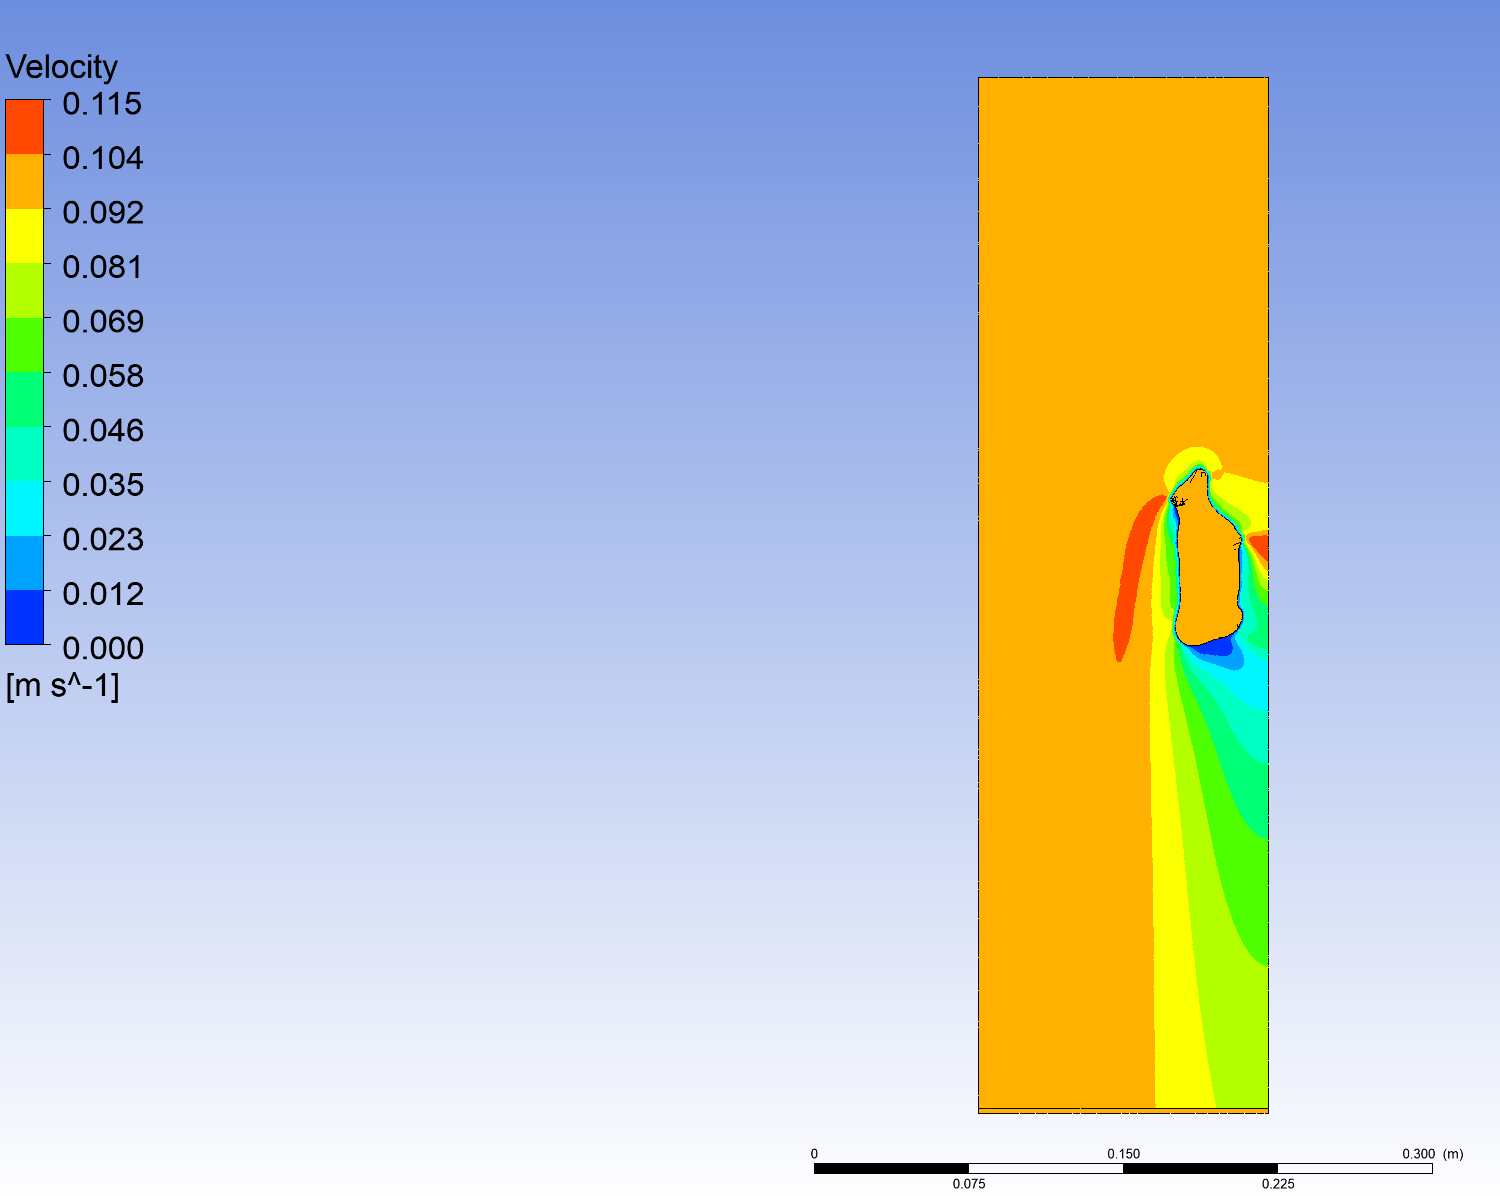
\includegraphics[width=0.5\textwidth]{Unbenannt.PNG}
    \caption{Druckverteilung uber die Symetrieflache}
    \label{fig:p}
\end{figure}


\subsection{Netzfeinheit}
Die Netzfeinheit wird bei jedem neuen Import/Export neu definiert. Um das Modell sehr gut abzubilden, ist eine Netzfeinheit von 0.2 mm nötig. In Abbildung \ref{fig:02mesh} ist diese Feinheit zu sehen. Um mit der limitierten Hardware des VDIs ein Ergebnis erzielen zu können, musste eine Netzfeinheit von 2 mm gewählt werden.  In Abbildung \ref{fig:netz} ist diese Feinheit zu sehen. Die sehr hohe Auflösung des ursprünglichen 3D-Scans stellt eine erhebliche Herausforderung für eine Simulation dar.

\begin{figure}[h]
    \centering
    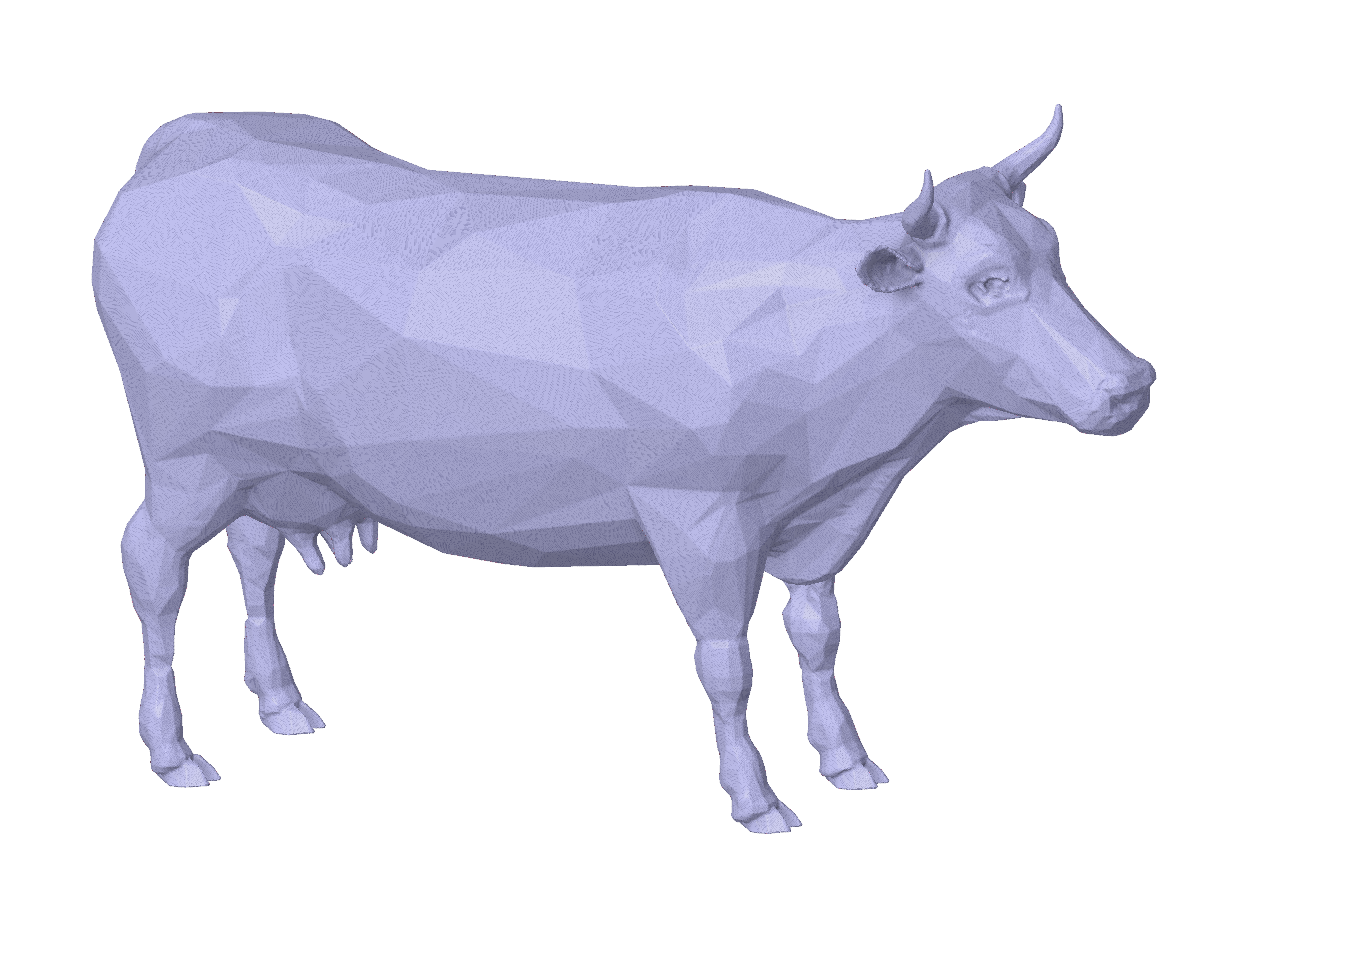
\includegraphics[width=0.5\textwidth]{cowremesh.PNG}
    \caption{Orginaldatai nach Shrinkwrap, mit Netzfeinheit 0.2 mm}
    \label{fig:02mesh}
\end{figure}


\begin{figure}[h]
    \centering
    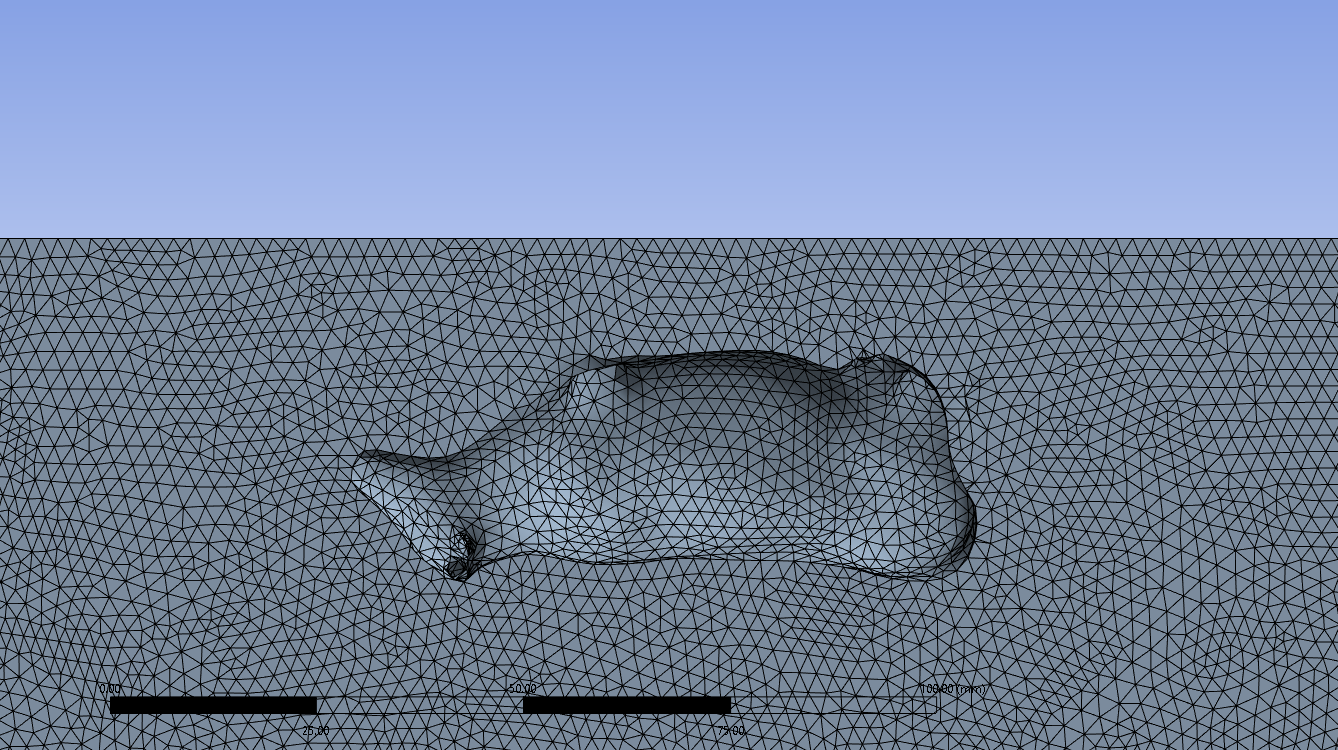
\includegraphics[width=0.5\textwidth]{nwtz.PNG}
    \caption{Simuliertes Netz, suboptimal aber konstant}
    \label{fig:netz}
\end{figure}

\section{Ergebnisse}
Es wird ein \( c_d original \) Wert von 0.88 und ein \( c_d scan \) von 0.91 simuliert. Die Werte sind in der gleichen Größenordnung wie die Handrechnung mit \( c_d kugel \) und das ist alles, was der theoretische Physiker braucht.

\subsection{Plausibilität}
Die Vergleichbarkeit des Originals mit dem Scan ist schwierig, da sowohl das Original als auch der Scan durch mehrere Programme transformiert wurden. Aber es zeigt trotzdem, wie gut ein \textit{gratis} 3D-Scanner sein kann, den man immer in der Hosentasche hat.

In der Literatur \href{https://www.youtube.com/watch?v=FDG3rUx00yQ}{Youtube} wurde das gleiche Orginal STL fur eine Berchenung benutzt und ein  \( c_d Youtube \) von 0.5 ermittelt.


\section{Fazit}
Es konnte in dieser selbst gestellten Testaufgabe ein Workflow entwickelt werden, um mit einem Photogrammetrie-3D-Scanner eine CFD-Simulation durchzuführen. Die größte Herausforderung des Workflows ist die Inkompatibilität der verschiedenen 3D-Dateitypen.

Die Simulation leidet an Turbulenzen, so konnten keine exakten Werte für den Luftwiderstand einer Kuh berechnet werden. Die beiden Simulationen und die Handrechnung sind in der gleichen Größenordnung, somit kann in der theoretischen Physik ohne Probleme die Annahme getroffen werden, dass eine Kuh eine Kugel ist.


\end{document}
